\documentclass[../structure.tex]{subfiles}
%\usepackage{../mypkg}
\begin{document}
\chapter{Background}
The human brain, which is the focus of our work in this thesis, is the central organ of the human nervous system. It is made up of two main components, namely, gray matter and white matter. Researchers have discerned a great deal about gray and white matter and distinct brain regions through autopsies and imaging techniques. The study of the human brain in diseased states or under conditions associated with brain damage have resulted in major insights into this complex organ.

\section{Brain Anatomy :Fiber Pathways}
	 \textbf{White matter} areas in the central nervous system are made up of myelinated axons, also known as tracts or fiber pathways \cite{Blumenfeld2010}. Fiber pathways are composed of bundles which connect various gray matter areas of the brain together and carry nerve impulses between neurons. Myelin acts as an insulator allowing electrical signals to jump rather than course through axons, increasing the speed of transmission of all nerve signals through a phenomenon known as saltatory conduction \cite{Klein2008}.
%	\\Long thought to be passive tissue, white matter affects learning and brain functions, modulates the distribution of action potentials, and acts as a relay and coordinator of communication between different brain regions \cite{Fields2008}.
	
	The human brain consists of the following tracts on both the left and right sides:


	\begin{figure}[h!]
	\centering
	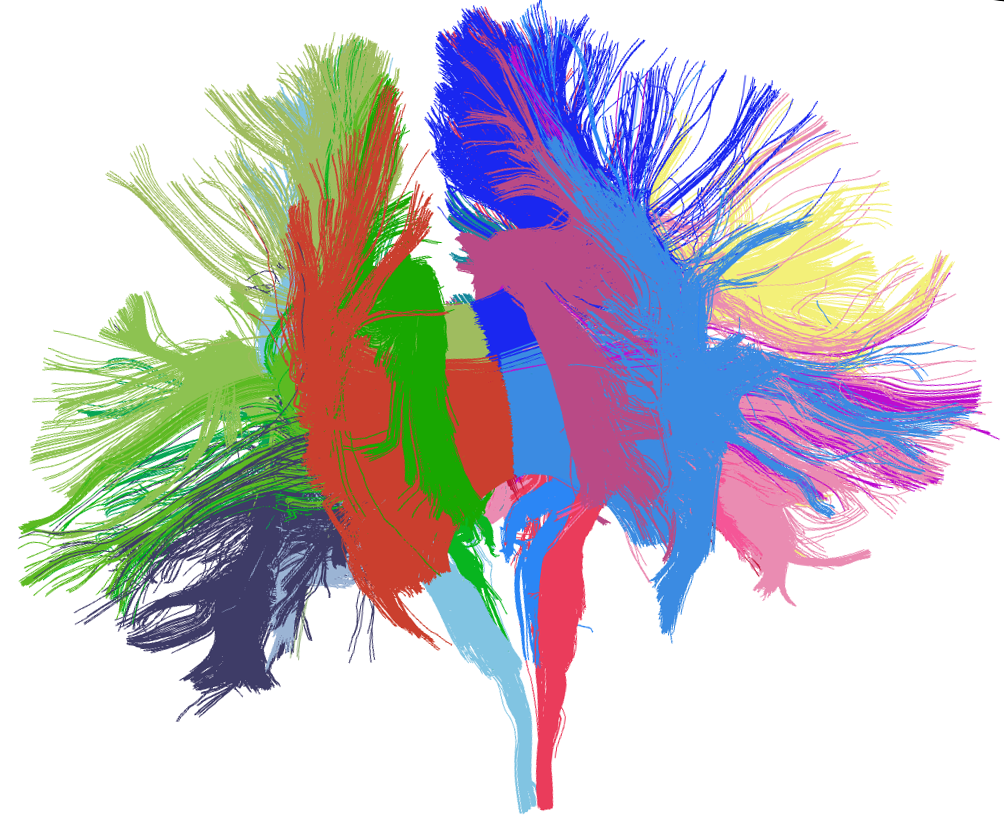
\includegraphics[scale=0.4]{000_all_brain}
	\captionsetup{justification=centering}
	\caption{The Human Brain Fiber Pathway}
	\label{fig:all_brain}
	\end{figure}
	
	\textbf{Anterior Thalamic Radiation} \\
	Anterior thalamic radiation (ATR) is a nerve fiber bundle that connects the anterior nuclear group of the thalamus and the midline nuclear group of the thalamus with the frontal lobe through the anterior thalamic peduncle, the anterior limb of the internal capsule and other parts of the cerebral white matter \cite{Washington1994}\cite{Grimm2018}. Abnormalities in ATR have a possible link with cognitive abnormalities and symptoms in schizophrenia\cite{Mamah2010}.	\\
		

	\textbf{Corpus Callosum } \\
	The corpus callosum is one of the largest transverse fibre and white matter tracts in the brain that links the cerebral cortex of the left and the right cerebral hemisphere. This region of the brain is divided into an anterior portion called the \textit{genu}, the \textit{rostrum} which is continuous with the lamina terminalis, a posterior structure known as the \textit{splenium} and in between its anterior and posterior portions lies the \textit{trunk/body}.\\


		\textbf{Cingulum}  \\
		Cingulum (Cing)is a collection of white matter fibres that connects portions of the parietal lobe, cingulate gyrus and prefrontal cortex with the parahippocampal gyrus and adjacent structures of the temporal lobe that always pass through the cingulum bundle  \cite{Washington1994}. It is described as a C shaped structure from various brain images that wraps around the frontal lobe to the temporal lobe above the corpus callosum. The posterior cingulate and anterior cingulate are two primary parts of the cingulate cortex that are related to cognitive functions and emotion,  especially apathy and depression respectively \cite{JaredTanner2010}.\\
		
		
	\textbf{Corticospinal Tract } \\	
		The corticospinal tract (CST) plays an important role in cortical control of spinal cord activity. It is a major tract for motor function. The CST originates from the secondary motor area, the parietal cortex, and the primary motor cortex. CST estimation and 3D visualization can be performed using diffusion tensor tractography, a technique derived from diffusion tensor imaging (DTI) \cite{Seo2013}.\\
		
		
		\textbf{Fornix (Fornix)} \\		
	The fornix, a discrete white matter tract bundle located on the medial aspects of the cerebral hemispheres is critical for normal cognitive functioning. It carries signals from the hippocampus to the hypothalamus which begins in the hippocampus on each side of the brain. The Fornix can be identified and segmented by using diffusion tensor imaging. Functionally relevant alterations in forniceal integrity in health and disease states can be identified using a technique called quantitative fiber tracking \cite{Thomas2011}.\\

	
		\textbf{Inferior Fronto-occipital Fasciculus} \\		
		The inferior fronto-occipital fasciculus (IFOF)  was the one of the first association fiber systems to be recognized in the human brain \cite{Wu2016}. It passes through a depth of temporal lobe and insula, connecting the occipital cortex, temporo-basal areas, and superior parietal lobe to the frontal lobe \cite{PDD2015} . \\

				
		\textbf{Inferior Longitudinal Fasciculus}\\		
		Inferior Longitudinal Fasciculus (ILF) is an associative white matter pathway that connects the occipital and temporal-occipital areas of the brain to the anterior temporal areas.  Sudden disruption of the ILF by neurologic insult is mainly associated with  neuropsychological impairments of visual cognition such as visual agnosia, prosopagnosia, and alexia \cite{Herbet2018}. The ILF is in direct contact with few other association tracts, namely, the uncinate fasciculus, the inferior fronto-occipital fasciculus (IFOF), the long and posterior/vertical segments of the arcuate fasciculus and the vertical occipital fasciculus of Wernicke.\\

		

		\textbf{Superior Longitudinal Fasciculus}\\			
		The superior longitudinal fasciculus (SLF) is a fiber pathway in the cerebral white matter that connect temporo-parietal language regions to ipsilateral frontal and opercular areas \cite{Madhavan2014}. It comprises three subcomponents namely, SLF I, II, and III linking the parietal lobe association cortices with the frontal lobe. The arcuate fasciculus (AF), once thought to be synonymous, appears to be separate and distinct from the SLF \cite{Schmahmann2006}.\\
		
		
		\textbf{Ventral Tegmental Area}\\
		The ventral tegmental area (VTA) is situated adjacent to the substantia nigra in the midbrain and is one of the major dopaminergic areas in the brain. Although there is no clear anatomical separation between the VTA and the substantia nigra, there are areas that seem to differ slightly. Together with an integral part of a network of structures, this region is known as the reward system involved in reinforcing behavior. The VTA is also thought to play a major role in motivation, reward, emotional and cognitive processes. This area of the brain is activated with the experience of something rewarding and may in turn be necessary for the development of addiction. Other than addiction, the VTA is involved in pathophysiology of disorders as is the case with schizophrenia, where dopaminergic neurons in the VTA have been proposed to play a role, and attention-deficit hyperactivity disorder (ADHD), which has been linked to low dopamine activity in the VTA \cite{Kalivas1993}.\\
	
\section{Fiber Tracking with Diffusion MRI}
Non-invasive delineation in the white matter with fiber tracking increases the clinical applications and offers potential for neuroscience. Therefore, it is becoming an important tool for surgery planning, visualization and localization of important white matter pathways. Fiber tracking also plays an important role in the field of \textit{connectomics} that generates and studies comprehensive maps of the complex network of connections in the brain \cite{Jeurissen2017}.

\subsection{Diffusion MRI}
A special type of MRI sequence which is sensitive to the random microscopic motion of water molecules is used in diffusion MRI. A directional dependence on this motion is introduced by coherent arrangement of fibres because water molecules are less hindered along the length of the fibres versus their movement in a perpendicular orientation. The measurement of a signal for each imaging voxel with a number of non-collinear orientations with diffusion MRI leads to the assessment of the local fiber orientations throughout the tissue of interest which can then be pieced together to infer long-range pathways connecting distant regions of the brain, a process called fiber tracking or fiber tractography.

The dMRI technology ease the clinical application and understanding brain anatomy and functions, that because its ability to delineate white brain fiber pathways. To be able to understand how the brain works as one unit, we need to understand the activity of cortical regions and physical connection that transfer the information between regions \cite{Jeurissen2017}.

\section{Image Registration}
Image registration (IR), also known as alignment or absolute orientation, is crucial in several fields such as computer vision , medicine and remote sensing. 3D IR is an approach to solve existing variants of the problem \cite{Cordon2006}. It is the process of transforming different batches of data such as multiple photographs from different sensors, times, depths or views into one coordinate system. Medical image registration of data from the same patient taken at different time spans for change detection or tumor monitoring involves elastic registration also called non rigid registration to deal with deformation of the bundles.

If we have two objects and we need to align them, that means we should reduce the distance between them by making one object fixed and move the other one to the closest distance. This simple form of alignment is called rigid transformation If we were to add scaling, then it would be called non-rigid transformation and would extend to the size of the object as well. Due to its fundamental importance in computer vision, it is a necessary step in many different applications for instance, object recognition, tracking, range data fusion, graphics, medical image alignment, robotics and structural bioinformatics \cite{Li2007}.

		\subsection{Iterative closest point}
		
		Iterative closest point (ICP) is an existing method for point cloud registration.  It estimates the motion parameters by minimizing the Euclidean distances between two or more point clouds. Point-to-point correspondences is the most common type so far whereas point-to-plane ICP estimates the parameters by minimizing the orthogonal distance between the points in one point cloud and the local planes in the other.
		
In ICP (in our case) one points cloud (i.e., vertex cloud), or target, is kept fixed, while the template, is transformed to best match the target. The algorithm iteratively checks the transformation (a combination of translation, rotation and scaling) required to minimize a distance from the template to the target points cloud \cite{Zhang1994}.

		 \subsubsection{Least squares (LSQR)}
		
		 LSQR is an iterative method to solve complex linear systems of equations and least square problems to approximate the solution. It allows the choice of an arbitrary initial vector for the solution subspace. The number of iterations required to reach a certain accuracy depends on the scaling of the problem ($ ||Ax-b||^2 $) \cite{Paige1982a}.
% please add the equations

\section{Principal component analysis Transformation}

Principal component analysis (PCA) is an orthogonal linear transformation for better alignment and orientation of the objects before performing the ICP.  It transforms the data into a system of coordination so that the greatest variance by any projection of the data comes to lie on the first few coordinates or first few components \cite{Jolliffe2002}.


\section{K-Dimensional (KD) Tree}

A K-D Tree is a binary search tree where each node is a K-Dimensional point in space which is used for nearest neighbor searches and each level of the tree splits all children along a specific dimension, using a hyperplane perpendicular to the corresponding axis (see figure \{\ref{fig:k_d_tree}\}.

\begin{figure}[h!]
	\centering
	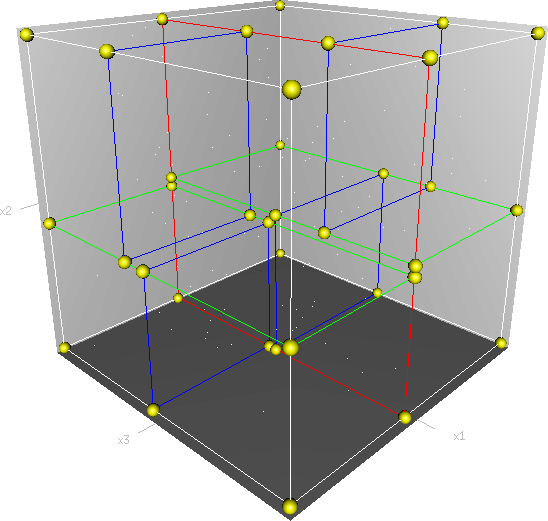
\includegraphics[scale=0.5]{005_3dtree}
	\captionsetup{justification=centering}
	\caption{K-D tree in 3D coordinate splitting the space \cite{Wikipedia2006}.}
	\label{fig:k_d_tree}
\end{figure}
\end{document}

